%
% This document is licensed under the
%
%   Creative Commons Attribution-Noncommercial-Share Alike
%
% license. Please see LICENSE file for details.
%

\documentclass{InsightArticle}

\usepackage[dvipdfmx]{graphicx}
\usepackage{url}
\usepackage{textcomp}

\usepackage[dvipdfmx,
bookmarks,
bookmarksopen,
backref,
colorlinks,linkcolor={blue},citecolor={blue},urlcolor={blue},
]{hyperref}


\title{Structural MRI Unwarping Using CMTK\footnote{This document is licensed under
    the Creative Commons Attribution License Version 3.0.}}

\release{1.2}

\author{Torsten Rohlfing}
\authoraddress{Neuroscience Program, SRI International, Menlo Park, CA}

\begin{document}

\maketitle

\ifhtml
\chapter*{Front Matter\label{front}}
\fi


\begin{abstract}
\noindent This document describes the workflow for unwarping structural MR
images, in particular $T_1$-weighted SPGR and MP-RAGE scans, using reference
scans of the Magphan\textsuperscript{\textregistered} EMR051 Quantitative
Imaging Phantom (a.k.a. ADNI Phantom) and the tools of the Computational
Morphometry Toolkit (CMTK).
\end{abstract}

\tableofcontents

\clearpage
\section{Introduction}

Nonlinear distortions and drift of scale calibration can severely confound
imaging-based studies, especially when run on multiple scanners or even at
multiple imaging sites. 

The Magphan\textsuperscript{\textregistered} EMR051 Quantitative Imaging
Phantom (also known as the ``ADNI Phantom'' after the Alzheimer's Disease
Neuroimaging Initiative) provides a technical solution for detecting, and
ultimately correcting, the effects of nonlinearity as well as drift over time,
whether on a single scanner or across devices.

Unfortunately, software tools to make practical use of the phantom are not
freely available~\cite{GuntBernBoro:2009} (see also
\cite{RohlPoli:2012}).

We describe in this article for the first time a workflow implementing the
correction of scanner miscalibration and nonlinearities {\em using only freely
  available data and software tools.} Example image data is provided with the
article. Source code for all software tools is available from
\url{http://nitrc.org/projects/cmtk/}.

\section{What You Need and Where You Get It}

We will assume you already have an MR scanner. If not, pick up a used one on
eBay. Make sure you keep an eye on the shipping charges.

\subsection{Structural Imaging Phantom}

You will need the ``Magphan\textsuperscript{\textregistered} EMR051
Quantitative Imaging Phantom'' (also known as ``The ADNI
Phantom''~\cite{GuntBernBoro:2009}),
\url{http://www.phantomlab.com/products/magphan_adni.php}. Photos of one such
phantom are shown in Fig.~\ref{fig:Phantom}.

\begin{figure}[tbp]
\begin{center}
\setlength\tabcolsep{1mm}
\begin{tabular}{ccc}
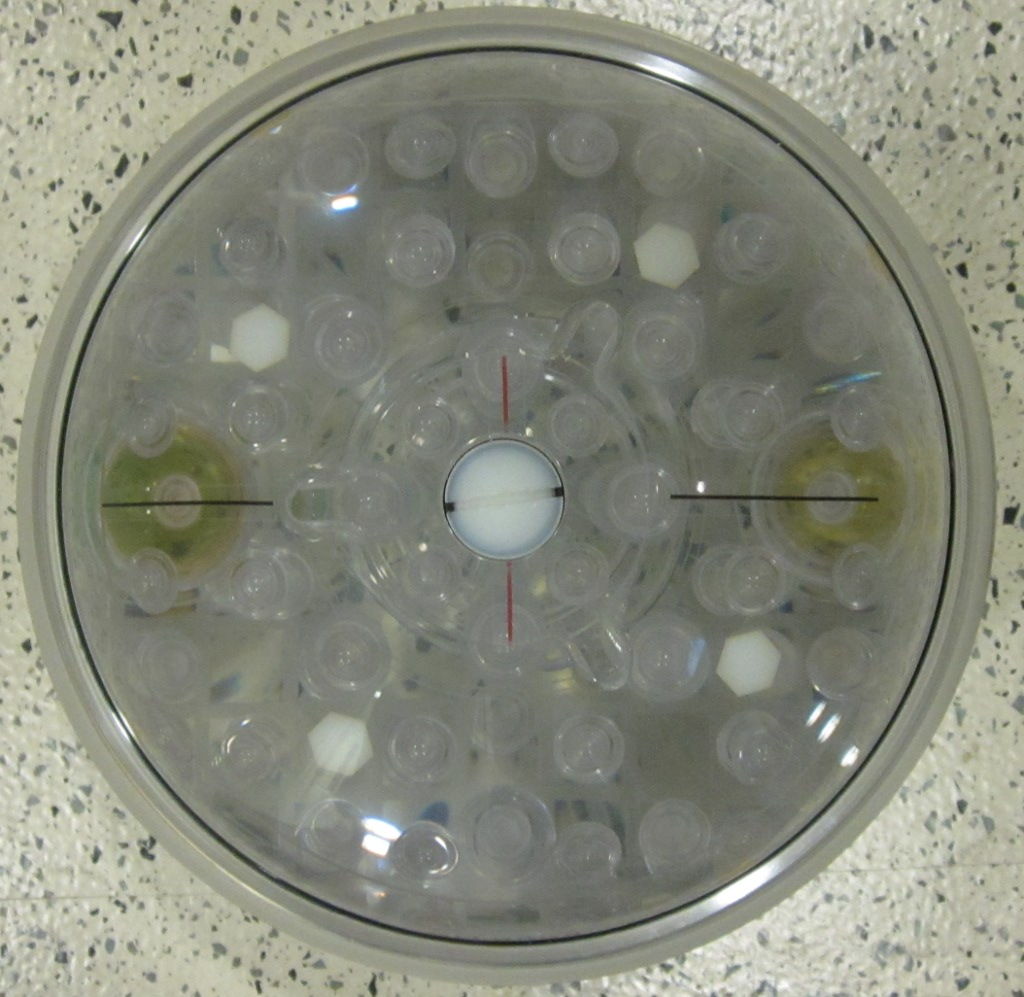
\includegraphics[height=.3\linewidth]{eps/magphanAP} &
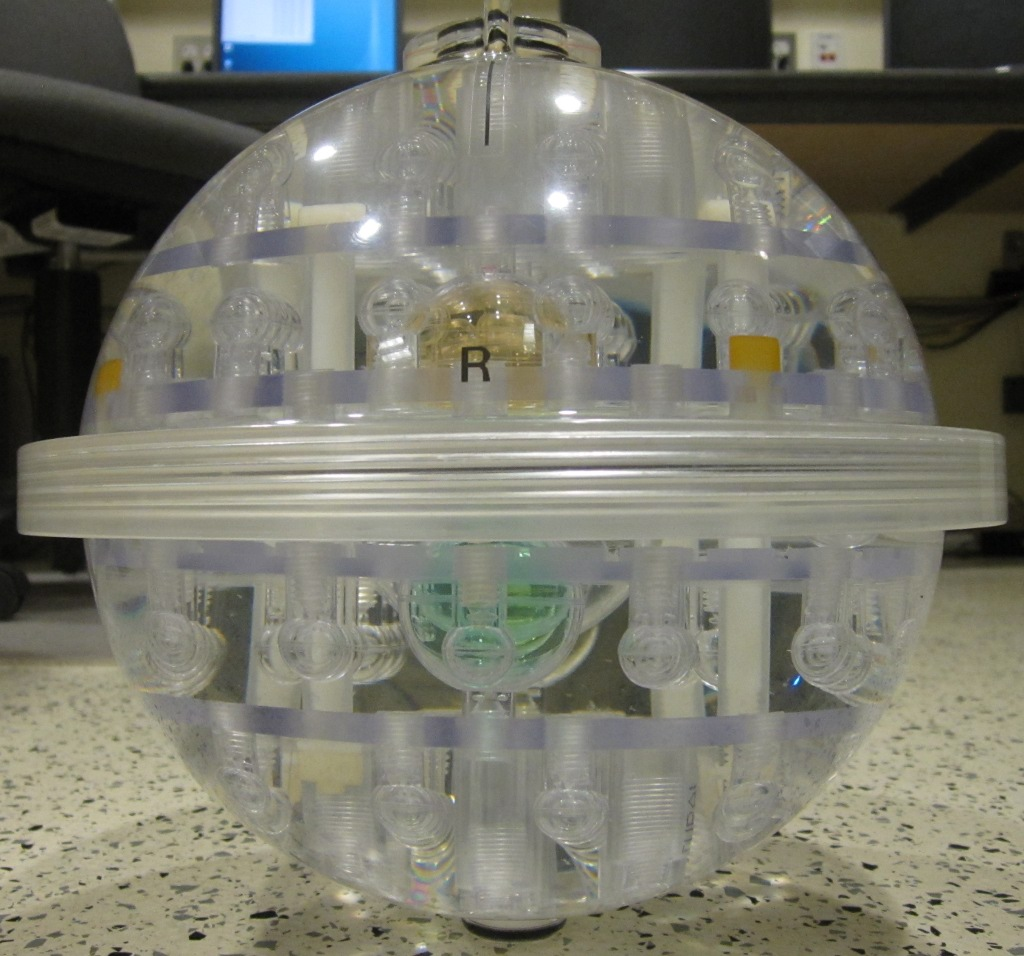
\includegraphics[height=.3\linewidth]{eps/magphanRL} &
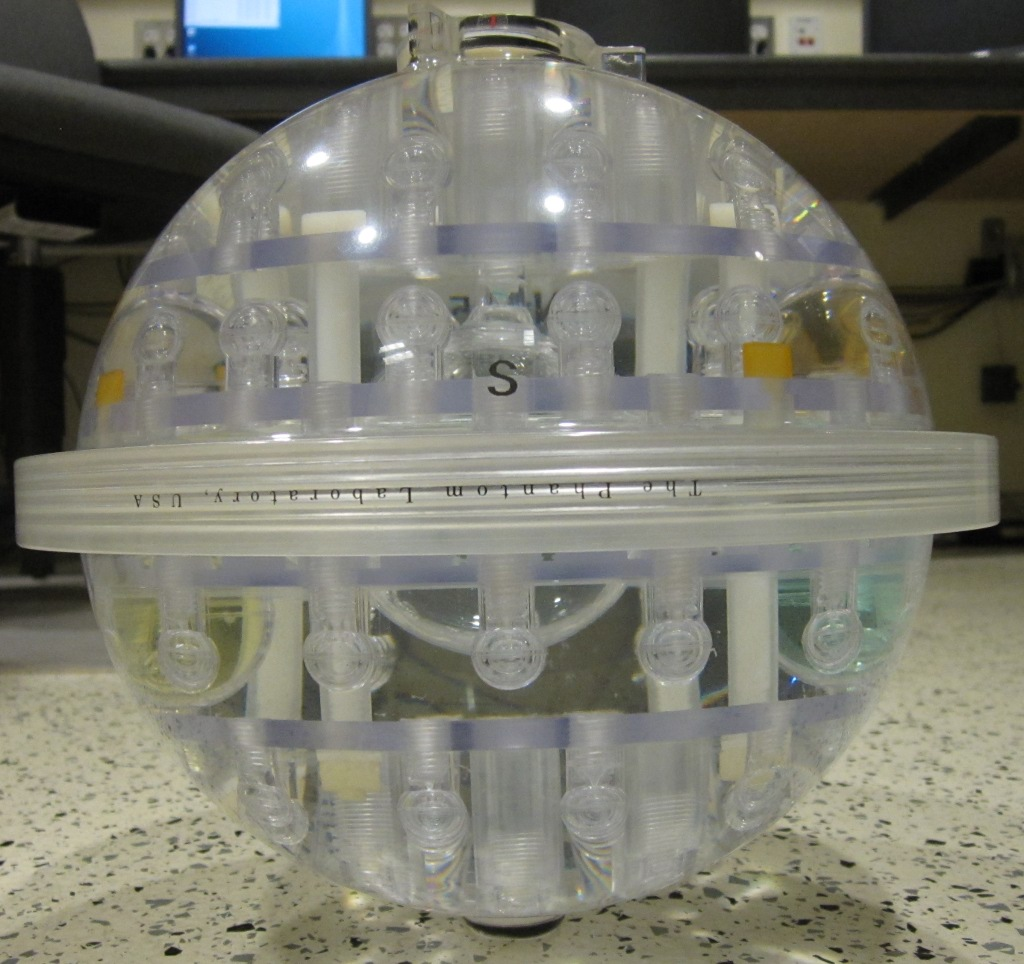
\includegraphics[height=.3\linewidth]{eps/magphanSI}
\end{tabular}
\end{center}
\caption{The Magphan\textsuperscript{\textregistered} EMR051 Quantitative
Imaging Phantom, seen from ``anterior,'' ``right,'' and ``superior''
direction (in ``patient coordinates,'' pictures from left to right).}
\label{fig:Phantom}
\end{figure}

The phantom can be purchased from the manufacturer, The Phantom Laboratory,
P.O. Box 511, Salem, NY, 12865-0511 USA. These are expensive -- hope you saved
some cash when you bought your scanner.

\subsection{CMTK}

Unlike the previous two items, The Computational Morphometry Toolkit (CMTK) is
{\bf free}, and that's as in both free beer and free speech. CMTK is available
both in source code, licensed under the GPLv3, and as pre-compiled binary
distributions from \url{http://nitrc.org/projects/cmtk/}. If you are using
NeuroDebian, you can also install CMTK directly.

We shall assume that CMTK has been installed such that its tools can be run as
\begin{verbatim}
cmtk <tool> <arg1> <arg2> ...
\end{verbatim}

{\bf You will need CMTK release 2.2.0 or later.} Earlier versions do not
  support phantom detection of landmark-based nonlinear deformations.

\section{Step-by-Step}

\subsection{Imaging}

The imaging phantom should be placed in the scanner according to manufacturer
instructions and $T_1$-weighted images should be acquired using the
site-preferred imaging sequence (e.g., SPGR or MP-RAGE). 

{\bf It is important to make sure that the entire phantom is contained within
  the acquisition field of view. Add slices if necessary.}

Example DICOM images of the phantom acquired with ``sagittal'' slice
orientation and full coverage are shown in Fig.~\ref{fig:PhantomDICOM}.

\begin{figure}[tbp]
\centerline{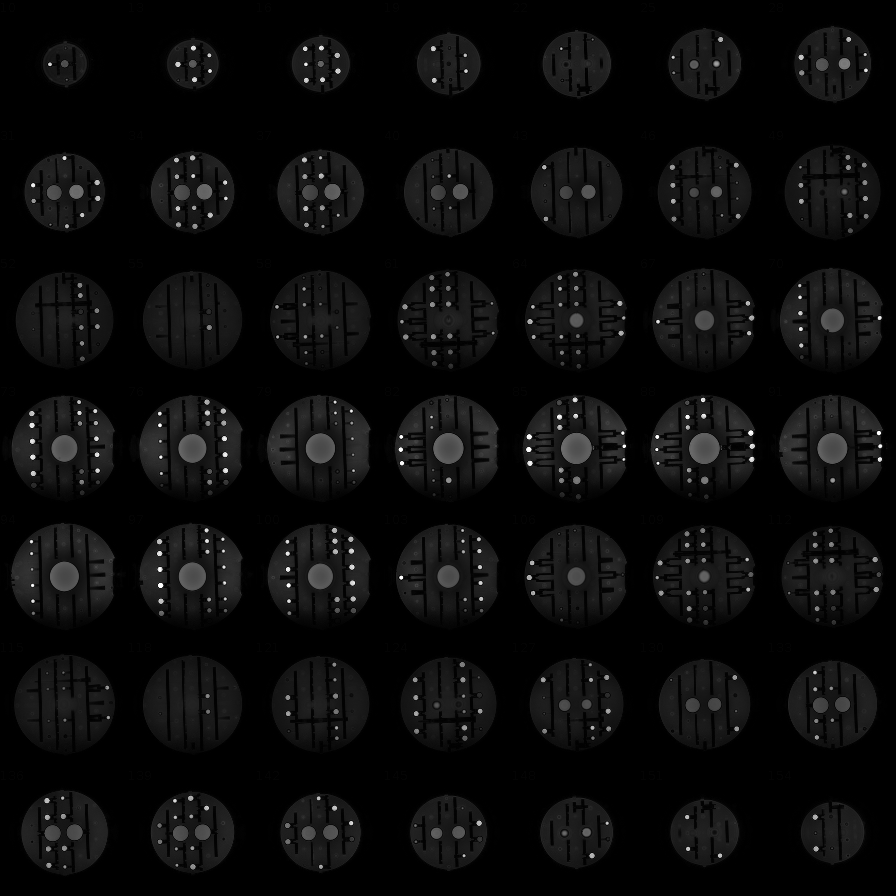
\includegraphics[width=.99\linewidth]{eps/magphan_dicom}}
\caption{Thumbnails of selected DICOM images acquired using SPGR acquisition
  on a GE MRI scanner (total number of slices in the acquisition was 176).}
\label{fig:PhantomDICOM}
\end{figure}

\subsection{DICOM Image Stacking}

Assume that the DICOM files containing the phantom images are stored in the
``\texttt{dicom/}'' directory. These are stacked into a 3D image in
NIFTI-format using the following CMTK command:
\begin{verbatim}
cmtk dcm2image -O phantom.nii dicom/
\end{verbatim}
Make sure only the DICOM files of the actual structural scans are in the
``\texttt{dicom/}'' directory, that is, not additional files such as scout
images\footnote{Otherwise, you can change the output file name to
  ``\texttt{phantom\%n.nii}'', which will result in multiple, numbered output
  images. You will then need to identify the correct one.}.

While CMTK supports a number of file formats, {\bf only NIFTI or NRRD format
  should be used for storing the phantom image.} The same is true for any
patient images to be unwarped. The reason for this limitation is that, of the
supported formats, only NIFTI and NRRD preserve the physical scanner
coordinates at which the images were acquired. This information is absolutely
necessary to determine the correct spatial relationship between phantom and
subject images. Without establishing this relationship, images cannot be unwarped.

\subsection{Phantom Detection}

Next, run the phantom image through the CMTK phantom detection tool. (For
hands-on testing, we are providing a NIFTI image of an actual SPGR phantom
scan with this article.)
\begin{verbatim}
cmtk detect_adni_phantom phantom.nii phantom.xml
\end{verbatim}
This will produce an XML file, ``\texttt{phantom.xml}'' containing, among
other information, the expected as well as detected locations of the centers
of all landmark spheres in the phantom. These locations provide the basis for
image unwarping. (An example of a generated XML file with a detailed
description of its contents can be found in Appendix~\ref{sec:ExampleXML})

To verify landmark locations, the phantom detection tool can optionally write
a label image matching the input image, in which the volume of each detected
phantom sphere is marked with a unique label. To this end, add
``\texttt{--write-labels labels.nii}'' to the above command line to produce
the labels file. See Fig.~\ref{fig:PhantomLabels} for an example of three
orthogonal slices from a phantom image with corresponding labeled spheres.

\begin{figure}[tbp]
\begin{center}
\setlength\tabcolsep{0.5mm}
\begin{tabular}{cc}
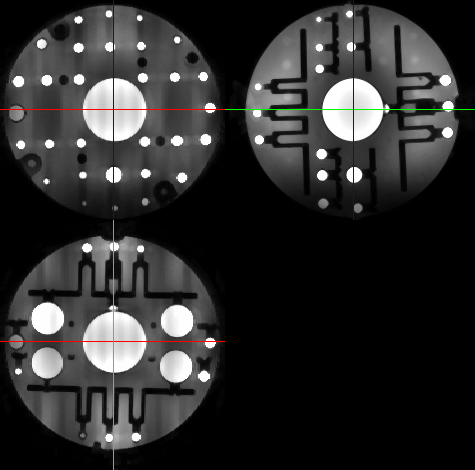
\includegraphics[width=.49\linewidth]{eps/phantom-labels-spgr} &
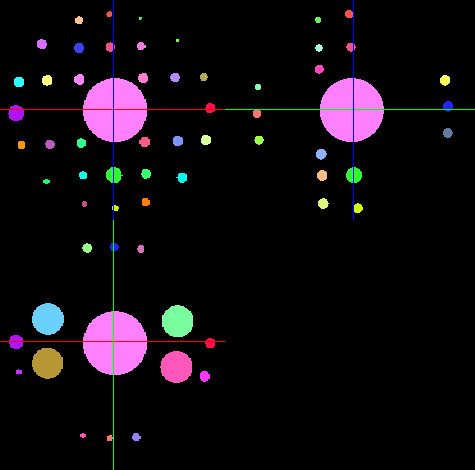
\includegraphics[width=.49\linewidth]{eps/phantom-labels}
\end{tabular}
\end{center}
\caption{Triplanar view of an SPGR image of the
Magphan\textsuperscript{\textregistered} EMR051 Quantitative Imaging Phantom
(left) and color-coded label map of phantom spheres detected by CMTK's
\texttt{detect\_adni\_phantom} tool.}
\label{fig:PhantomLabels}
\end{figure}

\subsection{Create Unwarping Transformation}

From the phantom description file, we can create an unwarping transformation
using the following CMTK command (to be entered on a single command line):
\begin{verbatim}
cmtk unwarp_image_phantom --final-cp-spacing 40 --levels 2 \
  phantom.xml phantom.nii unwarp.xform
\end{verbatim} 
This will generate a nonrigid transformation,
``\texttt{phantom\_warp.xform},'' in the space of the image
``\texttt{phantom.nii}.'' If a subject image, ``\texttt{subject.nii},'' is to
be unwarped, the command should be changed to (again entered on a single
command line):
\begin{verbatim}
cmtk unwarp_image_phantom --final-cp-spacing 40 --levels 2 \
  phantom.xml subject.nii unwarp.xform
\end{verbatim}

{\bf Note that a separate transformation must be created for every
  image to be unwarped, as each image has different physical coordinates.}

For now, the only supported representation for the unwarping transformation is
a B-spline free-form deformation~\cite{RuecSonoHaye:1999}, which requires
specification of a final control point spacing (here: 40\,mm) and is improved
by specifying also a number of multi-resolution levels for the spline fitting
process (here: 2 levels)~\cite{LeeWolbShin:1997}. Future versions of CMTK will
implement a thin-plate spline, in which each landmark will be used directly as
a control point.

\subsection{Correction With and Without Unwarping}

Using the deformation field fitted to the phantom landmark locations, the
phantom image can be unwarped as follows (entering the command on a single
command line):
\begin{verbatim}
cmtk reformatx --sinc-cosine -o unwarped.nii --floating phantom.nii \
  phantom.nii unwarp.xform
\end{verbatim} 
The phantom image, ``\texttt{phantom.nii},'' is listed twice
because it is both the floating (moving) and the reference (fixed)
image. Again, if a separate subject image is to be unwarped, the command
changes to
\begin{verbatim}
cmtk reformatx --sinc-cosine -o unwarped.nii --floating subject.nii \
  subject.nii unwarp.xform
\end{verbatim}

{\bf But do you really want to unwarp the image in the first place?}

Here's something to consider --- unwarping the image, phantom or subject,
requires interpolation and thus introduces smoothing, even though we are using
a sinc-kernel above. That's fine if you really need to know what anatomy is
exactly where, say to use the unwarped image for guiding implantation of a
deep-brain stimulator. {\bf (Except, it is not fine, because CMTK is not FDA
approved, so don't do it!)}

But what if you only want to unwarp the image to get the correct tissue or
region volumes somewhere down your processing pipeline? Then you might
actually be making things worse, for example for tissue segmentation, by
blurring the image ever so slightly.

Instead, what you really want to know is how the volume of each pixel changes
due to distortion so you can compute correct region and tissue volumes. Well,
we can do that without interpolation.

What we need for this correct is a map that tells us, for each pixel, how much
larger (or smaller) its volume really is, relative to the ideal volume as
prescribed in the imaging protocol. Mathematically speaking, we need the map
of Jacobian determinants of the inverse unwarping transformation in the
coordinate space of the acquired image. 

CMTK can give us this exact type of map using the following command (here, for
a subject image, but analogous for the phantom image itself if you care):
\begin{verbatim}
cmtk reformatx -o pxvolume.nii subject.nii unwarp.xform --jacobian \
  --inverse unwarp.xform
\end{verbatim}
Equivalently, we can use the following two commands to avoid numerical
inversion of the nonrigid transformation:
\begin{verbatim}
cmtk reformatx -o temporary.nii subject.nii --jacobian unwarp.xform
cmtk imagemath --in temporary.nii --one-over --out pxvolume.nii
\end{verbatim}
This makes use of the fact that the Jacobian determinant of forward and
inverse transformations are related by 
$$J_{T^{-1}}(T(\vec{x})) = 1/J_{T}(\vec{x})$$
for a transformation $T$ and any location $\vec{x}$. The former command above
computes the left-hand side of this equation, whereas the latter two-command
sequence computes its right-hand side.

Either way, the resulting image, ``\texttt{pxvolume.nii},'' contains at each
pixel the true volume of that pixel. By multiplying these values with tissue
volumes resulting from segmentation of the original image, we can obtain
distortion-corrected volumes {\em without actually unwarping and thus blurring
the original image.}

\section{Concluding Remarks}

At the time of writing, several of the software tools described herein (CMTK's
``\texttt{detect\_adni\_phantom}'' and ``\texttt{unwarp\_phantom\_image}''
tools) are still considered work-in-progress. We are making these tools and
this article available to provide the community with an opportunity to
evaluate our software in a timely fashion. Production use, however, it not
recommended at this time.

\section*{Acknowledgments}

Despite the name ``ADNI Phantom'' none of the materials used in this article
and none of the phantom-related code in CMTK make use of any ADNI data or
documentation, other than a cursory inspection of
Ref.~\cite{GuntBernBoro:2009}. In particular, the geometric specifications of
the phantom itself were derived from the phantom manual, available from
\url{http://www.phantomlab.com/library/pdf/magphan_adni_manual.pdf} The table
representing the geometry in CMTK's source code is included in
Appendix~\ref{sec:PhantomGeometry} and can be re-used under the terms of the
CC-BY-3.0 license.

{\bf Use of the materials and software tools described in this article does not
establish a requirement to acknowledge ADNI on the author list of subsequent
publications~\cite{RohlPoli:2012}.}

\bibliographystyle{UnwarpPhantom}
\bibliography{UnwarpPhantom}

\clearpage
\appendix

\section{Example Data}

This article is provided with an example image (``\texttt{phantom.nii.gz}'')
of an actual phantom. Running CMTK's phantom detection tool on this image
(with increased verbosity level for some intersting statistics) yields:
\begin{verbatim}
> cmtk detect_adni_phantom --verbose-level 2 --write-labels labels.nii \
    phantom.nii.gz phantom.xml
INFO: landmark fitting error average = 0.725241 maximum = 1.77297 
    maxErrName = 10mm_0_12 maxErrLabel = 19
INFO: detected and matched 160 out of 160 expected landmarks.
\end{verbatim}
This produces the phantom description file, ``\texttt{phantom.xml}.'' The
contents of this file are explained below in Appendix~\ref{sec:ExampleXML}.

We also see that all landmarks were successfully detected and the average
linear transformation fitting residual over all landmarks was 0.72\,mm. The
sphere with the maximum residual is ``\texttt{10mm\_0\_12},'' i.e., the 12th
of the 10\,mm spheres in Plane~0 of the phantom. (This sphere is labeled as
ROI~\#19 in the phantom label file, ``\texttt{labels.nii}.''

Using the XML phantom description, we can generate a nonrigid transformation
for phantom unwarping:
\begin{verbatim}
> cmtk unwarp_image_phantom --final-cp-spacing 40 --levels 2 phantom.xml \
    phantom.nii.gz phantom.xform
\end{verbatim}
Finally, we can use this transformation, ``\texttt{phantom.xform},'' to create
the unwarped phantom image:
\begin{verbatim}
cmtk reformatx -o unwarped.nii --floating phantom.nii.gz phantom.nii.gz \
    phantom.xform
\end{verbatim}

\section{Example XML Phantom File}
\label{sec:ExampleXML}

The \texttt{detect\_adni\_phantom} tool creates an XML file that contains a
description of the phantom detected in a given image. An example of the
contents of this file is shown below.

First, the file contains the XML header and the name of the represented
phantom:
\begin{verbatim}
<?xml version="1.0" encoding="utf-8"?>
<phantom>
<phantomType>MagphanEMR051</phantomType>
\end{verbatim}
Next, the file contains the estimated signal-to-noise ratio (based on the
phantom's SNR sphere) and four estimates of contrast-to-noise ratio (each
based on one of the four CNR spheres and its contrast relative to the SNR
sphere):
\begin{verbatim}
<snr>18.304893</snr>
<cnr>14.469221 35.670155 29.324328 28.170110</cnr>
\end{verbatim}
Following is the list of detected landmarks -- all coordinates are given in
physical image coordinates, derived ultimately from the DICOM headers but
represented in ``RAS'' coordinates (which means that $x$ and $y$ coordinates
are negative relative to DICOM's ``LPS'' coordinates):
\begin{verbatim}
<landmarkList coordinates="physical" space="RAS">
\end{verbatim} 
For each landmark, its unique name, expected location, detected
location, precision flag, and fitting residual are stored. The landmark name
is essentially arbitrary and based on the table of phantom landmarks as shown
in Appendix~\ref{sec:PhantomGeometry}.

The {\em expected location\/} is where the sphere center should be located in
the phantom image if the transformation between ideal phantom and image was
rigid (i.e., no scale, no shear, no nonlinearity). 

The {\em detected location\/} is where the sphere center was actually detected
in the image.

The {\em precision flag\/} specifies whether the ideal location of this sphere
should be considered as precise based on the phantom construction (e.g., the
SNR and CNR spheres have manufacturing tolerances that make their locations
unprecise). Only landmarks with this flag set to ``yes'' should be used for
regstration.

The {\em fitting residual\/} is the Euclidean distance between the detected
landmark location and the expected location according to a {\em linear fit\/}
of all landmarks. Note that here, the linear fit may include anisotropic scale
and shears, i.e., the residual is {\em not\/} simply the distance between
expected and detected location as stored in the file. The purpose of this
residual is to allow the transformation fitting tool to exclude outliers based
on a threshold of allowable residual.
\begin{verbatim}
        <landmark>
                <name>SNR</name>
                <expected>-2.081532 29.672649 -4.689435</expected>
                <detected>-4.846132 28.367746 -4.338875</detected>
                <isPrecise>no</isPrecise>
                <fitResidual>3.078036</fitResidual>
        </landmark>
        <landmark>
                <name>15mm@90mm</name>
                <expected>86.924671 28.899446 -7.279399</expected>
                <detected>87.598368 29.497402 -7.207202</detected>
                <isPrecise>no</isPrecise>
                <fitResidual>1.000909</fitResidual>
        </landmark>
        <landmark>
                <name>15mm@60mm</name>
                <expected>-3.739912 29.019053 -64.733024</expected>
                <detected>-3.855809 30.500179 -65.321349</detected>
                <isPrecise>no</isPrecise>
                <fitResidual>1.687546</fitResidual>
        </landmark>
        <landmark>
                <name>CNR-Orange</name>
                <expected>57.536139 46.089755 -5.790284</expected>
                <detected>58.235312 51.039218 -6.136547</detected>
                <isPrecise>no</isPrecise>
                <fitResidual>4.948012</fitResidual>
        </landmark>
        <landmark>
                <name>CNR-Red</name>
                <expected>-62.383089 43.226012 -2.446989</expected>
                <detected>-63.540399 48.950964 -2.568987</detected>
                <isPrecise>no</isPrecise>
                <fitResidual>5.653304</fitResidual>
        </landmark>
        <landmark>
                <name>CNR-Yellow</name>
                <expected>-61.699203 13.255542 -3.588586</expected>
                <detected>-62.273718 6.096574 -3.753603</detected>
                <isPrecise>no</isPrecise>
                <fitResidual>7.112524</fitResidual>
        </landmark>
        <landmark>
                <name>CNR-Green</name>
                <expected>58.220025 16.119286 -6.931881</expected>
                <detected>58.497813 9.654831 -7.491801</detected>
                <isPrecise>no</isPrecise>
                <fitResidual>6.319076</fitResidual>
        </landmark>
        <landmark>
                <name>10mm_0_01</name>
                <expected>-89.285621 28.732528 -32.248880</expected>
                <detected>-90.196775 29.579927 -32.380159</detected>
                <isPrecise>yes</isPrecise>
                <fitResidual>1.186873</fitResidual>
        </landmark>
        <landmark>
                <name>10mm_0_02</name>
                <expected>-87.561132 26.488978 27.684355</expected>
                <detected>-87.875622 26.872772 26.667286</detected>
                <isPrecise>yes</isPrecise>
                <fitResidual>0.919448</fitResidual>
        </landmark>

[more landmarks]

</landmarkList>
</phantom>
\end{verbatim}

\section{Phantom Geometry}
\label{sec:PhantomGeometry}

{\small
\begin{verbatim}
/*
 * Measurements were derived manually from the following document: 
 * http://www.phantomlab.com/library/pdf/magphan_adni_manual.pdf
 * They can, therefore, be used without reference to ADNI publications.
 */
const cmtk::MagphanEMR051::SphereEntryType 
cmtk::MagphanEMR051::SphereTable[cmtk::MagphanEMR051::NumberOfSpheres] =
{
  // 
  // LICENSING EXCEPTION
  //  Unlike the remainder of this file, the table of phantom sphere coordinates
  //  is licensed under the CC BY 3.0 license
  //  (https://creativecommons.org/licenses/by/3.0/us/)
  //
  // 1x 6.0cm SNR sphere
  { "SNR",        60, { 0.0, 0.0, 0.0 },      0.820, 282, Self::SPHERE_COLOR_NONE }, 
  // 2x 1.5cm spheres
  { "15mm@90mm",  15, {  89.0, -2.9,   0.0 },  0.820, 282, Self::SPHERE_COLOR_NONE },
  { "15mm@60mm",  15, {   0.0, -2.9, -60.0 },  0.820, 282, Self::SPHERE_COLOR_NONE },
  // 4x 3.0cm spheres -- estimated y coord's -- these are not marked in construction drawing
  { "CNR-Orange", 30, {  60.0,  15.0, 0 },    0.590, 450, Self::SPHERE_COLOR_ORANGE },
  { "CNR-Red",    30, { -60.0,  15.0, 0 },    0.430, 600, Self::SPHERE_COLOR_RED },   
  { "CNR-Yellow", 30, { -60.0, -15.0, 0 },    0.295, 750, Self::SPHERE_COLOR_YELLOW },
  { "CNR-Green",  30, {  60.0, -15.0, 0 },    0.220, 900, Self::SPHERE_COLOR_GREEN }, 
  // 158x 1.0cm spheres
  //   Plane 0
  //     outer ring
  { "10mm_0_01",  10, { -86.4, 0.0, -30.0 },  0.820, 282, Self::SPHERE_COLOR_NONE },
  { "10mm_0_02",  10, { -86.4, 0.0,  30.0 },  0.820, 282, Self::SPHERE_COLOR_NONE },
  { "10mm_0_03",  10, {  86.4, 0.0, -30.0 },  0.820, 282, Self::SPHERE_COLOR_NONE },
  { "10mm_0_04",  10, {  86.4, 0.0,  30.0 },  0.820, 282, Self::SPHERE_COLOR_NONE }, 
  { "10mm_0_05",  10, { -64.7, 0.0,  64.7 },  0.820, 282, Self::SPHERE_COLOR_NONE },
  { "10mm_0_06",  10, { -64.7, 0.0, -64.7 },  0.820, 282, Self::SPHERE_COLOR_NONE },
  { "10mm_0_07",  10, {  64.7, 0.0,  64.7 },  0.820, 282, Self::SPHERE_COLOR_NONE },
  { "10mm_0_08",  10, {  64.7, 0.0, -64.7 },  0.820, 282, Self::SPHERE_COLOR_NONE },
  { "10mm_0_09",  10, { -30.0, 0.0,  86.4 },  0.820, 282, Self::SPHERE_COLOR_NONE },
  { "10mm_0_10",  10, { -30.0, 0.0, -86.4 },  0.820, 282, Self::SPHERE_COLOR_NONE },
  { "10mm_0_11",  10, {  30.0, 0.0,  86.4 },  0.820, 282, Self::SPHERE_COLOR_NONE },
  { "10mm_0_12",  10, {  30.0, 0.0, -86.4 },  0.820, 282, Self::SPHERE_COLOR_NONE },
  { "10mm_0_13",  10, {   0.0, 0.0,  91.5 },  0.820, 282, Self::SPHERE_COLOR_NONE },
  { "10mm_0_14",  10, {   0.0, 0.0, -91.5 },  0.820, 282, Self::SPHERE_COLOR_NONE },
  //     middle ring
  { "10mm_0_15",  10, { -30.0, 0.0,  60.0 },  0.820, 282, Self::SPHERE_COLOR_NONE },
  { "10mm_0_16",  10, { -30.0, 0.0, -60.0 },  0.820, 282, Self::SPHERE_COLOR_NONE },
  { "10mm_0_17",  10, {  30.0, 0.0,  60.0 },  0.820, 282, Self::SPHERE_COLOR_NONE },
  { "10mm_0_18",  10, {  30.0, 0.0, -60.0 },  0.820, 282, Self::SPHERE_COLOR_NONE },
  { "10mm_0_19",  10, { -60.0, 0.0,  30.0 },  0.820, 282, Self::SPHERE_COLOR_NONE },
  { "10mm_0_20",  10, { -60.0, 0.0, -30.0 },  0.820, 282, Self::SPHERE_COLOR_NONE },
  { "10mm_0_21",  10, {  60.0, 0.0,  30.0 },  0.820, 282, Self::SPHERE_COLOR_NONE },
  { "10mm_0_22",  10, {  60.0, 0.0, -30.0 },  0.820, 282, Self::SPHERE_COLOR_NONE },
  //     inner ring
  { "10mm_0_23",  10, { -30.0, 0.0,  30.0 },  0.820, 282, Self::SPHERE_COLOR_NONE },
  { "10mm_0_24",  10, { -30.0, 0.0, -30.0 },  0.820, 282, Self::SPHERE_COLOR_NONE },
  { "10mm_0_25",  10, {  30.0, 0.0,  30.0 },  0.820, 282, Self::SPHERE_COLOR_NONE },
  { "10mm_0_26",  10, {  30.0, 0.0, -30.0 },  0.820, 282, Self::SPHERE_COLOR_NONE },
  //     single inferior mid-sagittal sphere
  { "10mm_0_27",  10, {   0.0, 0.0,  60.0 },  0.820, 282, Self::SPHERE_COLOR_NONE },
  //     single right sphere
  { "10mm_0_28",  10, { -91.5, 0.0,   0.0 },  0.820, 282, Self::SPHERE_COLOR_NONE },
  //   Plane 1
  //     mid-sagittal
  { "10mm_1_01",  10, {   0.0, -30.0,  40.0 },  0.820, 282, Self::SPHERE_COLOR_NONE },
  { "10mm_1_02",  10, {   0.0, -30.0, -40.0 },  0.820, 282, Self::SPHERE_COLOR_NONE },
  { "10mm_1_03",  10, {   0.0, -30.0,  86.5 },  0.820, 282, Self::SPHERE_COLOR_NONE },
  { "10mm_1_04",  10, {   0.0, -30.0, -86.5 },  0.820, 282, Self::SPHERE_COLOR_NONE },
  { "10mm_1_05",  10, {   0.0, -30.0,  60.0 },  0.820, 282, Self::SPHERE_COLOR_NONE },
  { "10mm_1_06",  10, {   0.0, -30.0, -60.0 },  0.820, 282, Self::SPHERE_COLOR_NONE },
  //     +- 30mm lateral
  { "10mm_1_07",  10, {  30.0, -30.0,  81.1 },  0.820, 282, Self::SPHERE_COLOR_NONE },
  { "10mm_1_08",  10, {  30.0, -30.0, -81.1 },  0.820, 282, Self::SPHERE_COLOR_NONE },
  { "10mm_1_09",  10, { -30.0, -30.0,  81.1 },  0.820, 282, Self::SPHERE_COLOR_NONE },
  { "10mm_1_10",  10, { -30.0, -30.0, -81.1 },  0.820, 282, Self::SPHERE_COLOR_NONE },
  { "10mm_1_11",  10, {  30.0, -30.0,  60.0 },  0.820, 282, Self::SPHERE_COLOR_NONE },
  { "10mm_1_12",  10, {  30.0, -30.0, -60.0 },  0.820, 282, Self::SPHERE_COLOR_NONE },
  { "10mm_1_13",  10, { -30.0, -30.0,  60.0 },  0.820, 282, Self::SPHERE_COLOR_NONE },
  { "10mm_1_14",  10, { -30.0, -30.0, -60.0 },  0.820, 282, Self::SPHERE_COLOR_NONE },
  { "10mm_1_15",  10, {  30.0, -30.0,  30.0 },  0.820, 282, Self::SPHERE_COLOR_NONE },
  { "10mm_1_16",  10, {  30.0, -30.0, -30.0 },  0.820, 282, Self::SPHERE_COLOR_NONE },
  { "10mm_1_17",  10, { -30.0, -30.0,  30.0 },  0.820, 282, Self::SPHERE_COLOR_NONE },
  { "10mm_1_18",  10, { -30.0, -30.0, -30.0 },  0.820, 282, Self::SPHERE_COLOR_NONE },
  //     +- 60mm lateral
  { "10mm_1_19",  10, {  60.0, -30.0,  30.0 },  0.820, 282, Self::SPHERE_COLOR_NONE },
  { "10mm_1_20",  10, {  60.0, -30.0, -30.0 },  0.820, 282, Self::SPHERE_COLOR_NONE },
  { "10mm_1_21",  10, { -60.0, -30.0,  30.0 },  0.820, 282, Self::SPHERE_COLOR_NONE },
  { "10mm_1_22",  10, { -60.0, -30.0, -30.0 },  0.820, 282, Self::SPHERE_COLOR_NONE },
  //     +- 61mm lateral
  { "10mm_1_23",  10, {  61.0, -30.0,  61.0 },  0.820, 282, Self::SPHERE_COLOR_NONE },
  { "10mm_1_24",  10, {  61.0, -30.0, -61.0 },  0.820, 282, Self::SPHERE_COLOR_NONE },
  { "10mm_1_25",  10, { -61.0, -30.0,  61.0 },  0.820, 282, Self::SPHERE_COLOR_NONE },
  { "10mm_1_26",  10, { -61.0, -30.0, -61.0 },  0.820, 282, Self::SPHERE_COLOR_NONE },
  //     +- 81.1mm lateral
  { "10mm_1_27",  10, {  81.1, -30.0,  30.0 },  0.820, 282, Self::SPHERE_COLOR_NONE },
  { "10mm_1_28",  10, {  81.1, -30.0, -30.0 },  0.820, 282, Self::SPHERE_COLOR_NONE },
  { "10mm_1_29",  10, { -81.1, -30.0,  30.0 },  0.820, 282, Self::SPHERE_COLOR_NONE },
  { "10mm_1_30",  10, { -81.1, -30.0, -30.0 },  0.820, 282, Self::SPHERE_COLOR_NONE },
  //     +- 86.5mm lateral
  { "10mm_1_31",  10, {  86.5, -30.0,   0.0 },  0.820, 282, Self::SPHERE_COLOR_NONE },
  { "10mm_1_32",  10, { -86.5, -30.0,   0.0 },  0.820, 282, Self::SPHERE_COLOR_NONE },
  //   Plane 1b
  //     +- 15mm lateral
  { "10mm_1b_01", 10, {  15.0,  29.1,  45.0 },  0.820, 282, Self::SPHERE_COLOR_NONE },
  { "10mm_1b_02", 10, {  15.0,  29.1,  65.0 },  0.820, 282, Self::SPHERE_COLOR_NONE },
  { "10mm_1b_03", 10, {  15.0,  29.1,  85.2 },  0.820, 282, Self::SPHERE_COLOR_NONE },
  { "10mm_1b_04", 10, {  15.0,  29.1, -45.0 },  0.820, 282, Self::SPHERE_COLOR_NONE },
  { "10mm_1b_05", 10, {  15.0,  29.1, -65.0 },  0.820, 282, Self::SPHERE_COLOR_NONE },
  { "10mm_1b_06", 10, {  15.0,  29.1, -85.2 },  0.820, 282, Self::SPHERE_COLOR_NONE },
  { "10mm_1b_07", 10, { -15.0,  29.1,  45.0 },  0.820, 282, Self::SPHERE_COLOR_NONE },
  { "10mm_1b_08", 10, { -15.0,  29.1,  65.0 },  0.820, 282, Self::SPHERE_COLOR_NONE },
  { "10mm_1b_09", 10, { -15.0,  29.1,  85.2 },  0.820, 282, Self::SPHERE_COLOR_NONE },
  { "10mm_1b_10", 10, { -15.0,  29.1, -45.0 },  0.820, 282, Self::SPHERE_COLOR_NONE },
  { "10mm_1b_11", 10, { -15.0,  29.1, -65.0 },  0.820, 282, Self::SPHERE_COLOR_NONE },
  { "10mm_1b_12", 10, { -15.0,  29.1, -85.2 },  0.820, 282, Self::SPHERE_COLOR_NONE },
  //     +- 40mm lateral
  { "10mm_1b_13", 10, {  40.0,  29.1,  15.0 },  0.820, 282, Self::SPHERE_COLOR_NONE },
  { "10mm_1b_14", 10, {  40.0,  29.1, -15.0 },  0.820, 282, Self::SPHERE_COLOR_NONE },
  { "10mm_1b_15", 10, { -40.0,  29.1,  15.0 },  0.820, 282, Self::SPHERE_COLOR_NONE },
  { "10mm_1b_16", 10, { -40.0,  29.1, -15.0 },  0.820, 282, Self::SPHERE_COLOR_NONE },
  //     +- 45mm lateral
  { "10mm_1b_17", 10, {  45.0,  29.1,  45.0 },  0.820, 282, Self::SPHERE_COLOR_NONE },
  { "10mm_1b_18", 10, {  45.0,  29.1, -45.0 },  0.820, 282, Self::SPHERE_COLOR_NONE },
  { "10mm_1b_19", 10, { -45.0,  29.1,  45.0 },  0.820, 282, Self::SPHERE_COLOR_NONE },
  { "10mm_1b_20", 10, { -45.0,  29.1, -45.0 },  0.820, 282, Self::SPHERE_COLOR_NONE },
  { "10mm_1b_21", 10, {  45.0,  29.1,  65.0 },  0.820, 282, Self::SPHERE_COLOR_NONE },
  { "10mm_1b_22", 10, { -45.0,  29.1, -65.0 },  0.820, 282, Self::SPHERE_COLOR_NONE },
  { "10mm_1b_23", 10, {  45.0,  29.1, -73.9 },  0.820, 282, Self::SPHERE_COLOR_NONE },
  { "10mm_1b_24", 10, { -45.0,  29.1,  73.9 },  0.820, 282, Self::SPHERE_COLOR_NONE },
  //     +- 64.5mm lateral
  { "10mm_1b_25", 10, {  64.5,  29.1, -45.0 },  0.820, 282, Self::SPHERE_COLOR_NONE },
  { "10mm_1b_26", 10, { -64.5,  29.1,  45.0 },  0.820, 282, Self::SPHERE_COLOR_NONE },
  //     +- 73.9mm lateral
  { "10mm_1b_27", 10, {  73.9,  29.1,  45.0 },  0.820, 282, Self::SPHERE_COLOR_NONE },
  { "10mm_1b_28", 10, { -73.9,  29.1, -45.0 },  0.820, 282, Self::SPHERE_COLOR_NONE },
  //     +- 85.2mm lateral
  { "10mm_1b_29", 10, {  85.2,  29.1,  15.0 },  0.820, 282, Self::SPHERE_COLOR_NONE },
  { "10mm_1b_30", 10, {  85.2,  29.1, -15.0 },  0.820, 282, Self::SPHERE_COLOR_NONE },
  { "10mm_1b_31", 10, { -85.2,  29.1,  15.0 },  0.820, 282, Self::SPHERE_COLOR_NONE },
  { "10mm_1b_32", 10, { -85.2,  29.1, -15.0 },  0.820, 282, Self::SPHERE_COLOR_NONE },
  //   Plane 2
  //     +- 15mm lateral
  { "10mm_2_01",  10, {  15.0, -60.0,  15.0 },  0.820, 282, Self::SPHERE_COLOR_NONE },
  { "10mm_2_02",  10, {  15.0, -60.0, -15.0 },  0.820, 282, Self::SPHERE_COLOR_NONE },
  { "10mm_2_03",  10, { -15.0, -60.0,  15.0 },  0.820, 282, Self::SPHERE_COLOR_NONE },
  { "10mm_2_04",  10, { -15.0, -60.0, -15.0 },  0.820, 282, Self::SPHERE_COLOR_NONE },
  { "10mm_2_05",  10, {  15.0, -60.0,  45.0 },  0.820, 282, Self::SPHERE_COLOR_NONE },
  { "10mm_2_06",  10, {  15.0, -60.0, -45.0 },  0.820, 282, Self::SPHERE_COLOR_NONE },
  { "10mm_2_07",  10, { -15.0, -60.0,  45.0 },  0.820, 282, Self::SPHERE_COLOR_NONE },
  { "10mm_2_08",  10, { -15.0, -60.0, -45.0 },  0.820, 282, Self::SPHERE_COLOR_NONE },
  { "10mm_2_09",  10, {  15.0, -60.0,  67.3 },  0.820, 282, Self::SPHERE_COLOR_NONE },
  { "10mm_2_10",  10, {  15.0, -60.0, -67.3 },  0.820, 282, Self::SPHERE_COLOR_NONE },
  { "10mm_2_11",  10, { -15.0, -60.0,  67.3 },  0.820, 282, Self::SPHERE_COLOR_NONE },
  { "10mm_2_12",  10, { -15.0, -60.0, -67.3 },  0.820, 282, Self::SPHERE_COLOR_NONE },
  //     +- 45mm lateral
  { "10mm_2_13",  10, {  45.0, -60.0,  15.0 },  0.820, 282, Self::SPHERE_COLOR_NONE },
  { "10mm_2_14",  10, {  45.0, -60.0, -15.0 },  0.820, 282, Self::SPHERE_COLOR_NONE },
  { "10mm_2_15",  10, { -45.0, -60.0,  15.0 },  0.820, 282, Self::SPHERE_COLOR_NONE },
  { "10mm_2_16",  10, { -45.0, -60.0, -15.0 },  0.820, 282, Self::SPHERE_COLOR_NONE },
  //     +- 48.7mm lateral
  { "10mm_2_17",  10, {  48.7, -60.0,  48.7 },  0.820, 282, Self::SPHERE_COLOR_NONE },
  { "10mm_2_18",  10, {  48.7, -60.0, -48.7 },  0.820, 282, Self::SPHERE_COLOR_NONE },
  { "10mm_2_19",  10, { -48.7, -60.0,  48.7 },  0.820, 282, Self::SPHERE_COLOR_NONE },
  { "10mm_2_20",  10, { -48.7, -60.0, -48.7 },  0.820, 282, Self::SPHERE_COLOR_NONE },
  //     +- 67.3mm lateral
  { "10mm_2_21",  10, {  67.3, -60.0,  15.0 },  0.820, 282, Self::SPHERE_COLOR_NONE },
  { "10mm_2_22",  10, {  67.3, -60.0, -15.0 },  0.820, 282, Self::SPHERE_COLOR_NONE },
  { "10mm_2_23",  10, { -67.3, -60.0,  15.0 },  0.820, 282, Self::SPHERE_COLOR_NONE },
  { "10mm_2_24",  10, { -67.3, -60.0, -15.0 },  0.820, 282, Self::SPHERE_COLOR_NONE },
  //   Plane 2b (same as Plane 2 but at y=+59.1)
  //     +- 15mm lateral
  { "10mm_2b_01", 10, {  15.0,  59.1,  15.0 },  0.820, 282, Self::SPHERE_COLOR_NONE },
  { "10mm_2b_02", 10, {  15.0,  59.1, -15.0 },  0.820, 282, Self::SPHERE_COLOR_NONE },
  { "10mm_2b_03", 10, { -15.0,  59.1,  15.0 },  0.820, 282, Self::SPHERE_COLOR_NONE },
  { "10mm_2b_04", 10, { -15.0,  59.1, -15.0 },  0.820, 282, Self::SPHERE_COLOR_NONE },
  { "10mm_2b_05", 10, {  15.0,  59.1,  45.0 },  0.820, 282, Self::SPHERE_COLOR_NONE },
  { "10mm_2b_06", 10, {  15.0,  59.1, -45.0 },  0.820, 282, Self::SPHERE_COLOR_NONE },
  { "10mm_2b_07", 10, { -15.0,  59.1,  45.0 },  0.820, 282, Self::SPHERE_COLOR_NONE },
  { "10mm_2b_08", 10, { -15.0,  59.1, -45.0 },  0.820, 282, Self::SPHERE_COLOR_NONE },
  { "10mm_2b_09", 10, {  15.0,  59.1,  67.3 },  0.820, 282, Self::SPHERE_COLOR_NONE },
  { "10mm_2b_10", 10, {  15.0,  59.1, -67.3 },  0.820, 282, Self::SPHERE_COLOR_NONE },
  { "10mm_2b_11", 10, { -15.0,  59.1,  67.3 },  0.820, 282, Self::SPHERE_COLOR_NONE },
  { "10mm_2b_12", 10, { -15.0,  59.1, -67.3 },  0.820, 282, Self::SPHERE_COLOR_NONE },
  //     +- 45mm lateral
  { "10mm_2b_13", 10, {  45.0,  59.1,  15.0 },  0.820, 282, Self::SPHERE_COLOR_NONE },
  { "10mm_2b_14", 10, {  45.0,  59.1, -15.0 },  0.820, 282, Self::SPHERE_COLOR_NONE },
  { "10mm_2b_15", 10, { -45.0,  59.1,  15.0 },  0.820, 282, Self::SPHERE_COLOR_NONE },
  { "10mm_2b_16", 10, { -45.0,  59.1, -15.0 },  0.820, 282, Self::SPHERE_COLOR_NONE },
  //     +- 48.7mm lateral
  { "10mm_2b_17", 10, {  48.7,  59.1,  48.7 },  0.820, 282, Self::SPHERE_COLOR_NONE },
  { "10mm_2b_18", 10, {  48.7,  59.1, -48.7 },  0.820, 282, Self::SPHERE_COLOR_NONE },
  { "10mm_2b_19", 10, { -48.7,  59.1,  48.7 },  0.820, 282, Self::SPHERE_COLOR_NONE },
  { "10mm_2b_20", 10, { -48.7,  59.1, -48.7 },  0.820, 282, Self::SPHERE_COLOR_NONE },
  //     +- 67.3mm lateral
  { "10mm_2b_21", 10, {  67.3,  59.1,  15.0 },  0.820, 282, Self::SPHERE_COLOR_NONE },
  { "10mm_2b_22", 10, {  67.3,  59.1, -15.0 },  0.820, 282, Self::SPHERE_COLOR_NONE },
  { "10mm_2b_23", 10, { -67.3,  59.1,  15.0 },  0.820, 282, Self::SPHERE_COLOR_NONE },
  { "10mm_2b_24", 10, { -67.3,  59.1, -15.0 },  0.820, 282, Self::SPHERE_COLOR_NONE },
  //   Plane 3
  { "10mm_3_01",  10, {  28.3, -82.2,  28.3 },  0.820, 282, Self::SPHERE_COLOR_NONE },
  { "10mm_3_02",  10, {  28.3, -82.2, -28.3 },  0.820, 282, Self::SPHERE_COLOR_NONE },
  { "10mm_3_03",  10, { -28.3, -82.2,  28.3 },  0.820, 282, Self::SPHERE_COLOR_NONE },
  { "10mm_3_04",  10, { -28.3, -82.2, -28.3 },  0.820, 282, Self::SPHERE_COLOR_NONE },
  { "10mm_3_05",  10, {   0.0, -88.0,  25.0 },  0.820, 282, Self::SPHERE_COLOR_NONE },
  { "10mm_3_06",  10, {   0.0, -88.0, -25.0 },  0.820, 282, Self::SPHERE_COLOR_NONE },
  { "10mm_3_07",  10, {  25.0, -88.0,   0.0 },  0.820, 282, Self::SPHERE_COLOR_NONE },
  { "10mm_3_08",  10, { -25.0, -88.0,   0.0 },  0.820, 282, Self::SPHERE_COLOR_NONE },
  { "10mm_3_09",  10, {   0.0, -89.5,   0.0 },  0.820, 282, Self::SPHERE_COLOR_NONE },
  //   Plane 3b
  { "10mm_3b_01", 10, {  28.3,  81.4,  28.3 },  0.820, 282, Self::SPHERE_COLOR_NONE },
  { "10mm_3b_02", 10, {  28.3,  81.4, -28.3 },  0.820, 282, Self::SPHERE_COLOR_NONE },
  { "10mm_3b_03", 10, { -28.3,  81.4,  28.3 },  0.820, 282, Self::SPHERE_COLOR_NONE },
  { "10mm_3b_04", 10, { -28.3,  81.4, -28.3 },  0.820, 282, Self::SPHERE_COLOR_NONE },
  { "10mm_3b_05", 10, {   0.0,  87.2,  25.0 },  0.820, 282, Self::SPHERE_COLOR_NONE },
  { "10mm_3b_06", 10, {   0.0,  87.2, -25.0 },  0.820, 282, Self::SPHERE_COLOR_NONE },
  { "10mm_3b_07", 10, {  25.0,  87.2,   0.0 },  0.820, 282, Self::SPHERE_COLOR_NONE },
  { "10mm_3b_08", 10, { -25.0,  87.2,   0.0 },  0.820, 282, Self::SPHERE_COLOR_NONE },
  { "10mm_3b_09", 10, {   0.0,  88.6,   0.0 },  0.820, 282, Self::SPHERE_COLOR_NONE }
  // 
  // END LICENSING EXCEPTION
  //
\end{verbatim}
}

\end{document}

